%------------------------------------------------
% Latex-Grundgerüst für Seminarausarbeitungen
%
% zu Erzeugen mit
%   pdflatex template.tex
%
% von Carsten Gutwenger
% angepasst von Igor Vatolkin
%------------------------------------------------

\documentclass[a4paper,12pt,twoside]{article}
% \usepackage[a4paper,left=3.5cm,right=2.5cm,bottom=3.5cm,top=3cm]{geometry}
\setlength{\headheight}{15pt}

% Encoding der .tex-Datei
% muss je nach Editor-Einstellungen eventuell angepasst werden!
%   latin1    Unix/Windows
%   ansinew   Alternative für Windows
%   applemac  Apple
%   utf8      Alternative für Unix/Windows/Apple
\usepackage[utf8]{inputenc}

\usepackage[T1]{fontenc}                                    % Unterstützung für Umlaute mit Fonts
\usepackage[pdftex]{graphicx,color}                         % Einbetten von Grafiken, Farbe
\usepackage[format=plain,small,bf,indention=7.5mm]{caption} % verbesserte Beschriftung von Abbildungen
\usepackage{subfig}                                         % subfigures
\usepackage{url}                                            % \url{}-Kommando
\usepackage{fancyhdr,float}                                 % Kopf-/Fußzeilen
\usepackage[pdftex,pdfpagelabels]{hyperref}                 % Hyperlinks im PDF
\usepackage{natbib,doi}                                     % Literaturverzeichnis, DOIs
\usepackage[section,boxed]{algorithm}                       % Floating-Umgebung für Algorithmen
\usepackage{algpseudocode}                                  % Pseudocode für Algorithmen
%\usepackage{commenting}

\captionsetup{farskip=10pt,topadjust=0pt,captionskip=10pt,nearskip=0pt,margin=10pt}

\pagestyle{fancy}
\fancyhead[LE,RO]{\thepage}
\fancyhead[RE]{\nouppercase{\slshape \leftmark}}
\fancyhead[LO]{\nouppercase{\slshape \rightmark}}
\fancyfoot[C]{}


\begin{document}

%------------------------------------------------
% Titelseite
%------------------------------------------------

\begin{titlepage}
\vspace*{-2cm}
\newlength{\links}
\setlength{\links}{-1.5cm} \sf \LARGE

\hspace*{\links}
\begin{minipage}{12.5cm}

\includegraphics[width=8cm]{RWTH_Logo_3.svg.png}
\end{minipage}

\vspace*{4cm}

\large
\begin{center}
{\Large Seminar work} \\[1ex]
{\LARGE\textbf{Generating music based on audio and text}}\\[3ex]
Max Kinsperger, 467539 - Felix Krückel, 454343 \\[1ex]
\today\\[7ex]
as part of seminar\\[1ex]
{\Large\textbf{Artificial Intelligence in Music Data Analysis}}\\[1ex]
organised by Dr.~Igor Vatolkin\\[1ex]
Summer term 2025
\end{center}

\vspace*{5cm}
\hspace*{\links}
\begin{minipage}[b]{15cm}
\normalsize \raggedright

\textbf{Based on:}\\
    Simon Rouard, Yossi Adi, Jade Copet, Axel Roebel, and Alexandre Défossez \\
    Audio Conditioning for Music Generation via Discrete Bottleneck Features \\
    ISMIR 2024
\end{minipage}

\vfill
\hspace*{\links}
\begin{minipage}[b]{8cm}
\normalsize \raggedright
RWTH Aachen\\
Computer Science 14\\
Artificial Intelligence Methodology\\
\url{https://www.aim.rwth-aachen.de/}
\end{minipage}

\end{titlepage}

%------------------------------------------------
% Inhaltsverzeichnis
%------------------------------------------------

\tableofcontents
\clearpage


%------------------------------------------------
% Einführung
%------------------------------------------------

\section{Introduction}

Literature reviews and critically thinking about past work are integral parts of a healthy scientific community.
Thus this work aims to reflect on the scientific value and methodological quality of work on audio conditioning in music generation by Rouard et. al.'s work \cite{rouardAudioConditioningMusic2024}.\\

The authors present to novel contributions aiming to allow high quality music generation based on a context containing both audio and text inputs. They specifically present an adaptation of an existing method creating "pseudowords", based on existing work in the computer vision domain \cite{galImageWorthOne2022}
and a novel method enabling fast inference for new audio samples, through lossy encoding of style features and an attention mechanism. \\ % \comment{Is attention the correct framing here? I'd guess this might create confusion.}

Section \ref{backgrounds} starts by describing backgrounds relevant for the experiments in section \ref{experiments}.
The following section \ref{discussion} and section \ref{summary} present and discuss the paper's main results.

\section{Backgrounds}\label{backgrounds}

Backgrounds here \\



For each background info, please provide only the most important details:
\begin{itemize}
    \item For which tasks can the method be applied?
    \item How is its working principle (a rough explanation)?
    \item Who has proposed it and when?
    \item Which pros and cons does it have?
\end{itemize}



Method here.\\

\begin{equation}
\mathcal S(q_1,...,q_{N}) = vol\left(\bigcup_{i=1}^{N}\ [q_i,{\bf r}]\right)
\label{eq:hypervolume}
\end{equation}

\begin{figure}[!h]
    \centering
    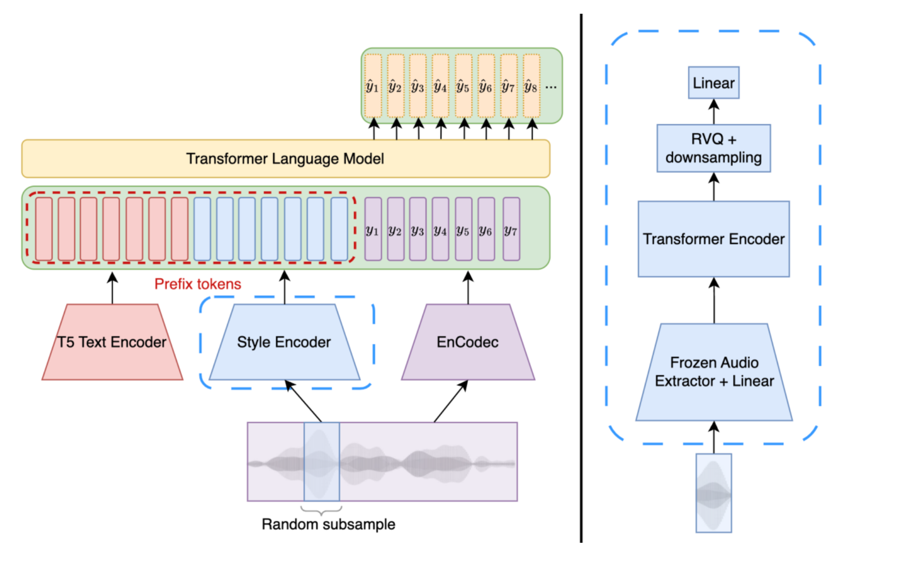
\includegraphics[width=0.9\textwidth]{1.png}
    \caption{Papers Figure 2}
    \label{Figure 1}
\end{figure}

\section{Experiments}\label{experiments}

Experiments here


\begin{table}[!h]


\caption{Comparison of methods}


\label{tab1}


\centering


\begin{tabular}{|p{2cm}|l|r|}
\hline
Algorithm & Dataset & Accuracy \\
\hline
Naive Bayes & DS10 & 22.14 \\
Naive Bayes & DS100 & 9.17 \\
Random \newline Forest & DS10 & 80.56 \\
Random \newline Forest & DS100 & 40.31 \\
\hline
\end{tabular}
\end{table}


\section{Discussion}\label{discussion}

Discussion

\subsection{Style encoding}
Why only 2-5s of subsample for style conditioning?

\subsection{Music generation speed}
The model takes roughly 3 min. to generate a 15s piece of music on an A10G GPU.

\subsection{Out of Training Distribution Generalization}
Music of Africa test.
Pfeifen

\subsection{Safety}
We believe AI development should follow a human centric approach and should be developed with rigorous . The authors did not perform safety

\section{Summary}\label{summary}

Summary.
%------------------------------------------------
% Literaturverzeichnis
%------------------------------------------------
\newpage
\bibliographystyle{plainnat}
\bibliography{literature}
\addcontentsline{toc}{section}{\bibname}


\end{document}
